\section{Background: Load Balancing}

Managing the load of a cluster of servers is a common problem in distributed computing systems.
Load-balancing policies typically rely on some notion of ``load'' of a server, such as the number of concurrently executing tasks, length of the task-queue, cpu-utilization, etc.
%
The first broad class is \emph{compute-oriented} load-balancers, typically used for short-running tasks and queries. 
Load-balancing for computational tasks is common in scenarios like web-clusters~\cite{karger1999web}. 
In these systems, the tasks can be executed on any server,  servers in a cluster are largely fungible, and the task performance largely depends on the server-specific cpu-utilization at the time.

Load-balancing techniques have received significant theoretical attention (especially using queuing theory), as well as many practical systems~\cite{decandia2007dynamo}. 
From a queuing theory perspective, policies such as least-work-left (LWL) and Join-Shortest-Queue (JSQ), have studied near-optimal load balancing for computing load-dependent workloads under a processor-sharing (PS) setting. 

Interestingly, load-balancing for \emph{data-oriented} systems, such as Content Delivery Networks (CDNs)~\cite{nygren2010akamai}, and distributed key-value stores (such as Amazon Dynamo~\cite{decandia2007dynamo}) must also balance the load on servers, but with data locality as a key requirement.
In this context, locality refers to requests for the same object being handled by the server, or the same subset of servers if the object is replicated. 
We find that FaaS load balancing requires and benefits from \emph{both} these objectives: minimizing computing load \emph{and} maximizing locality to reduce cold starts. 

\begin{comment}
However, combining compute-oriented load-balancing solutions 

In large clusters, consistent load information cannot always be assumed, and simple techniques work well in practice.
For instance, the power of two random choices, which schedules a task on the least loaded of two random servers. 

Queuing analysis?
- G/G/PS system. Greedy load balancing is sub-optimal.

Randomization and power of 2 choices is popular.

But arent locality aware.

Web server load balancing work. A Gandhi etc. 
\end{comment}

%\vspace*{-0.2cm}
\subsection{Consistent Hashing} 
\label{subsec:ch}

\begin{figure}
  \centering
  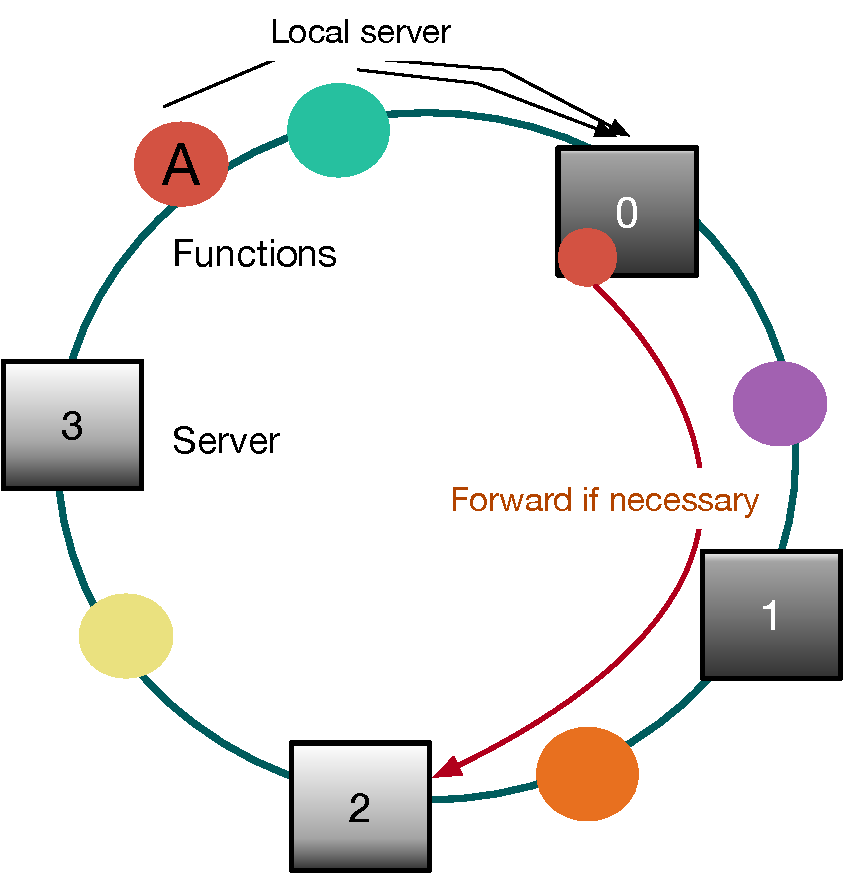
\includegraphics[width=0.7\textwidth]{chrlu/faaslb-osdi22/figs/ch-bl.pdf}
%  \vspace*{-0.2cm}
  \caption{Consistent hashing runs functions on the nearest clockwise server. Functions are forwarded along the ring if the server is overloaded.}
  \label{fig:ch}
%    \vspace*{-0.2cm}
\end{figure}

For data-oriented systems, a common technique to ensure locality is Consistent Hashing~\cite{karger1999web, karger1997consistent}.
Objects are mapped to servers based on some object id or key.
Consistent hashing preserves object-server mapping even in the face of server additions and removals, which improves locality.
%
Figure~\ref{fig:ch} provides an overview of consistent hashing. Both objects and servers are hashed to points on a ``ring'', and objects are assigned to the next server (in the clockwise direction) in the ring. 
Addition or removal of servers only affects the nearby objects by remapping them to the new next server in the ring.

OpenWhisk uses a modified consistent hashing algorithm for its default load balancer.
As functions are sent to servers, their expected memory footprint is added to a server-specific running counter of outstanding requests.
Upon completion the memory size of a function is decremented from that server's counter.
If the counter for a function's \quotes{home} server would exceed the assigned memory on the server it is forwarded along the ring.
%
The drawback of this policy, and consistent hashing as a whole, is that the performance can be affected by the relative popularities of the different objects.
A highly popular object can result in its associated server getting overloaded.
This problem is exacerbated in the case of FaaS functions, as we shall demonstrate in the next section. 
